\documentclass[runningheads,a4paper]{llncs}

\setcounter{tocdepth}{3}
\usepackage[portuguese]{babel}
\usepackage[utf8]{inputenc}
\usepackage{amssymb}
\usepackage{graphicx}
\usepackage{color}
\usepackage{soul}
\usepackage{hyperref}
\usepackage[normalem]{ulem}
\usepackage{threeparttable}
\usepackage{booktabs}
\usepackage[portuguese,ruled,lined]{algorithm2e}
\usepackage{algorithmic}
\usepackage{enumerate}
\usepackage{subcaption}
\usepackage{float}

\usepackage{url}
\urldef{\mails}\path|{nathmenini, serza.arnosti, jorge.inatel}@gmail.com|
\newcommand{\keywords}[1]{\par\addvspace\baselineskip
\noindent\keywordname\enspace\ignorespaces#1}

\graphicspath{ {imgs/} } % Path com imagens

\begin{document}

\mainmatter

\title{Estimação da Distância de Reversão de Genomas Baseada em Técnicas de Aprendizado de Máquina}

\titlerunning{Estimação da Distância de Reversão de Genomas}

\author{Nathalia Menini, Sergio Z. Arnosti e Jorge da Silva}

\institute{Instituto de Computação da Unicamp,\\
Av. Albert Einstein, 1251 - Cidade Universitária, Campinas - SP\\
\mails}

\maketitle

\begin{abstract}
A Biologia Computacional trouxe muitos avanços na tarefa de comparar dois genomas para se estudar as relações e a evolução entre os genes como, por exemplo, através da distância de rearranjo.
Neste trabalho, propõe-se a utilização de técnicas de Aprendizado de Máquina, como a Regressão Linear e Redes Neurais, com o objetivo de estimar a distância de reversão para permutações sem orientação de genes baseando-se em \textit{features} extraídas dessas. O treinamento dos algoritmos considerou permutações de tamanhos reduzidos e, posteriormente, verificou o desempenho em permutações maiores. Esses métodos foram comparados com algoritmos já estabelecidos na literatura como, por exemplo, o \textit{Selection Sort Using Reversals} e \textit{Greedy Reversal Sort}, bem como com a distância exata de reversão. Os resultados mostram que a utilização de Regressão Linear apresenta resultados melhores ou tão bons quanto o algoritmo \textit{Greedy Reversal Sort} (2-aproximação). Além disso, para as permutações de tamanho maior que 10, a Regressão Linear e Rede Neural se mostraram abordagens promissoras para a estimação de distância de reversão.
\keywords{genes, reversão, aprendizado de máquina, permutação, estimação, distância}
\end{abstract}

\section{Introdução}
\label{sec:1}

Comparar dois genomas é uma tarefa fundamental para se estudar as relações e a evolução entre os genes~\cite{Lou,daSilva}. Nesse caminho, a Biologia Computacional tem se apresentado como uma ótima aliada para os pesquisadores da área, tornando possível descobrir relações entre os genes que, para a percepção do ser humano, poderia ser muito difícil de detectar~\cite{daSilva}.

Nesse contexto, o conceito de \textit{rearranjo de genomas} se torna essencial. O rearranjo de genomas é uma mutação que ocorre nos genomas mitocondriais~\cite{Russel}, de modo que a ordem dos genes está em constante rearranjo. Desse modo, através da estimação da distância de rearranjo entre dois genes, a relação entre eles pode ser estimada~\cite{Pevzner}.

Um dos eventos de mutação mais comuns em genomas, conhecido como \textit{reversão}, ocorre quando um fragmento do filamento de DNA é revertido. Por outro lado, se dois fragmentos de DNA trocam de posições durante o processo de replicação (mas não sofrem reversão), temos um evento de mutação chamado de \textit{transposição}~\cite{daSilva}.

A área da Filogenia, que estuda a história evolutiva das relações entre espécies, depende fortemente do Principio da Parcimônia~\cite{Podani}. Basicamente, dado um conjunto de possíveis explicações para um fato, a explicação mais simples é a mais provável de estar correta. Como as mutações são relativamente raras de acontecer, quando os pesquisadores constroem uma árvore filogenética, eles tentam fazer com que as espécies tenham o menor número de antecessores possíveis, o que significa que é mais provável que duas espécies que possuem uma mesma característica tenham evoluído de um mesmo ancestral comum do que essa mesma característica ter evoluído duas vezes de espécies diferentes \cite{daSilva}.

Entretanto, determinar o número de mutações necessárias para um genoma se transformar em outro não é um problema fácil de se resolver~\cite{daSilva}. Mais especificamente, considerando a permutação identidade $\iota = (1,2,...,n)$ de tamanho $n$ como o genoma original, dada qualquer permutação $\pi$ de tamanho $n$, o problema consiste em construir um modelo capaz de calcular a distância de rearranjo de $\pi$ a $\iota$, em que são permitidas apenas operações de reversão.

Uma outra possível representação de genomas é utilizando a \textit{orientação} dos genes. Nesse caso, representamos o genoma com os símbolos $+$ ou $-$ para cada gene como, por exemplo, na permutação $(+1,-2,\cdots,-n)$. Na literatura, essa abordagem é conhecida como \textit{permutações com orientação de genes conhecida}. Por outro lado, se não temos informações sobre a orientação dos genes, os sinais são omitidos e a abordagem passa a ser chamada de \textit{permutação sem orientação de genes conhecida}. Este trabalho utilizará apenas a segunda abordagem, ou seja, sem orientação de genes~\cite{Setubal}. 

Novamente, determinar o número mínimo de reversões necessárias para um genoma se transformar em outro, considerando o contexto de permutações sem orientação, não é um problema fácil de ser resolvido, uma vez que foi provado ser um problema pertencente a classe NP-difícil~\cite{Caprara}.

Muitas abordagens já foram propostas para atacar esse problema como, por exemplo, Kececioglu e Sankoff em \cite{Kececioglu} propuseram um algoritmo de 2-aproximação que remove \textit{breakpoints} por reversão (o conceito de \textit{breakpoint} será descrito posteriormente), Bafna e Pevzner em \cite{Bafna} criaram o algoritmo de 1.75-aproximação utilizando grafos de reversão e Christie~\cite{Christie} apresentou um algoritmo com fator de aproximação 1.5. O atual estado da arte foi desenvolvido por Berman \textit{et al.} \cite{Berman}, que construiu um algoritmo de 1.375-aproximação. Além disso, Berman e Karpinski~\cite{Berman2}, mostraram que o problema da distância de reversão sem orientação é MAX-SNP-difícil. Abordagens utilizando algoritmos genéticos e técnicas de Aprendizado de Máquina (AM) também já foram propostas por Auyeung e Abraham em \cite{Auyeung} e da Silva \textit{et al.} em \cite{daSilva}, respectivamente.

Entretanto, a maioria dos algoritmos presentes na literatura buscam, além de encontrar a distância de reversão, encontrar também as reversões que transformam uma permutação em outra. Neste trabalho, propõe-se a utilização de técnicas de AM, como a Regressão Linear e Redes Neurais, com o objetivo de estimar a distância de reversão baseando-se em \textit{features} obtidas a partir da permutação, no contexto de permutações sem orientação. 

Em um primeiro momento, o foco será estimar a distância e não obter as reversões em si, uma vez que, em áreas como a filogenia, é fundamental obter uma métrica de distância entre objetos~\cite{Podani} e, quanto mais precisa for a métrica, melhor será a análise. Além disso, devido a dificuldade de obter dados da distância de reversão exata para permutações grandes, serão utilizados como dados para treinamento dos algoritmos propostos um \textit{dataset} com permutações de tamanhos reduzidos e, posteriormente, será verificado o desempenho em permutações maiores.

\section{Definições e Conceitos Básicos}
\label{sec:2}

Nessa seção, será explicada a operação de reversão no contexto de permutações sem orientação e, também, alguns conceitos utilizados para o protocolo de extração das \textit{features} utilizadas nos algoritmos de AM.

Os genomas podem ser representados por permutações ($n$-tuplas, em que $n$ é a quantidade de genes), em que cada gene é representado por um número e que todos os genes são diferentes um dos outros. Ou seja, uma permutação $\pi$ de tamanho $n$ é representada por $\pi=(\pi_1\ \pi_2\ \cdots \ \pi_n)$, com $\pi_i \in \{1,2,\cdots n\}$ e $\pi_i \neq \pi_j \iff i \neq j$. A \textit{permutação identidade}, como mencionada anteriormente, é definida como $\iota = (1\ 2\ \cdots n)$. A \textit{composição} entre duas permutações $\pi$ e $\sigma$ é dada por $\pi\sigma=(\pi_{\sigma_1}\ \pi_{\sigma_2} \cdots \pi_{\sigma_3})$. Definimos também o \textit{inverso} de uma permutação $\pi$ como $\pi^{-1}$, em que $\pi^{-1}\pi=\iota$.

A \textit{permutação extendida} de uma permutação $\pi=(\pi_1\ \pi_2\ \cdots \ \pi_n)$, denotada por $\pi_e$, é definida como $\pi_e=(0\ \pi_1\ \pi_2\ \cdots \ \pi_n \ n+1)$. A definição de permutação extendida é necessária para a descrição de operações que serão abordadas no decorrer do trabalho.

Dadas duas permutações $\pi$ e $\sigma$ e um conjunto de operações $\Sigma=\{\rho_1, \rho_2, \cdots, \rho_k \}$, o problema de transformar $\pi$ em $\sigma$ consiste em obter no menor número possível de operações de $\Sigma$ aplicada em $\pi$, tal que $\pi$ seja transformada em $\sigma$. O número de operações necessárias é chamado de distância entre $\pi$ e $\sigma$, representado por $d(\pi,\sigma)$. Para fins de notação, será utilizado $d(\pi,\iota)=d(\pi)$.

O problema de encontrar a distância entre as permutações $\pi$ e $\sigma$ é equivalente ao problema de encontrar a distância entre alguma permutação $\pi'$ e $\iota$, em que $\pi'=\sigma^{-1}\pi$. Ou seja, se queremos encontrar a distância entre $\pi$ e $\sigma$, equivale ao problema de ordenação de $\sigma^{-1}\pi$. Por exemplo, se considerarmos $\pi=(5\ 3\ 1\ 6\ 7\ 4\ 2)$ e $\sigma=(6\ 3\ 2\ 7\ 5\ 1\ 4)$, temos que $\sigma^{-1}=(6\ 3\ 2\ 7\ 5\ 1\ 4)$, o que faz com que $\pi'=\sigma^{-1}\pi=(5\ 2\ 6\ 1\ 4\ 7\ 3)$. Então, a distância entre $\pi$ e $\sigma$ equivale a distância de ordenação de $\pi'$.

% \begin{figure}
% 	\centering
% 	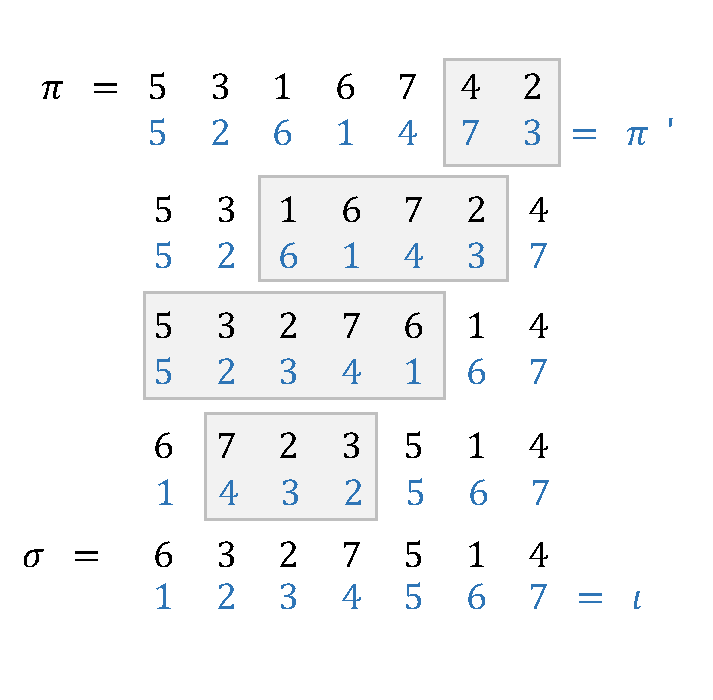
\includegraphics[height=6.2cm]{perms.pdf}
% 	\caption{Equivalência na distância entre $\pi$ e $\sigma$ com a distância entre $\pi'$ e $\iota$.}
% 	\label{fig:2}
% \end{figure}

\subsection{Reversões}

Uma operação de reversão $\rho_r(i,j)$, com $1 \leq i < j \leq n$ reverte um fragmento da permutação, ou seja, $\rho_r(i,j)$ aplicado em $\pi=(\pi_1\ \cdots \ \pi_{i-1}\ \underline{\pi_i \cdots \pi_j}\ \pi_{j+1} \ \cdots \ \pi_n)$ gera $\pi \rho_r(i,j) = (\pi_1\ \cdots \ \pi_{i-1}\ \underline{\pi_j \cdots \pi_i}\ \pi_{j+1} \ \cdots \ \pi_n)$.

Considere, por exemplo, $\pi=(1\ 4\ 3\ 2\ 6\ 7\ 5)$ e a operação de reversão $\rho_r(2,4)$. O resultado após aplicar essa operação é $\pi \rho_r(2,4)= (1\ \underline{2\ 3\ 4}\ 6\ 7\ 5)$.

\subsection{\textit{Breakpoints}}
\label{sec:breakpoints}

No contexto de operações de reversão, dada uma permutação estendida de $\pi$, um par de elementos $\pi_i$ e $\pi_{i+1}$, para $0\leq i \leq n$, é definido como uma adjacência se $|\pi_i - \pi_{i+1}| = 1$. Caso contrário, o par de elementos é chamado de \textit{breakpoint}. A permutação identidade é a única que não possui \textit{breakpoints} e a quantidade de \textit{breakpoints} de uma permutação é denotada por $b(\pi)$~\cite{daSilva,Jones}.

Como exemplo, dada a permutação $\pi = (0 \ 1 \ 2 \bullet 6 \ 5 \bullet 3 \ 4 \bullet 7)$, tem-se três \textit{breakpoints} -- destacados com o símbolo $\bullet$ : um entre os elementos 2 e 6, outro entre os elementos 5 e 3 e, por fim, entre os elementos 4 e 7.

\subsection{\textit{Strips}}
\label{sec:strips}

\textit{Strips} podem ser definidas como fragmentos de uma permutação que não apresentam \textit{breakpoints}. Mais precisamente, uma \textit{strip} $\pi[i \cdots j]$ é um trecho maximal em $\pi$ tal que todos os pares $(\pi_k, \pi_{k+1})$ são adjacências, para $i\leq k<j$~\cite{daSilva,Jones}.

Uma \textit{strip} $\pi[i \cdots j]$ é chamada descrescente se e somente se a sequência $\pi_i, \pi_{i+1},\cdots,\pi_{j-1},\pi_j$ for descrescente. As \textit{strips unitárias} são sempre definidas como descrescentes, com exceção das \textit{strips} formadas por $\pi_0$ e $\pi_{n+1}$ que são sempre crescentes. Por outro lado, se a sequência for crescente, a \textit{strip} é dita crescente. Considere que o símbolo $\rightarrow$ representa uma \textit{strip} crescente e $\leftarrow$ uma \textit{strip} decrescente, desse modo, temos que as \textit{strips} de $\pi$ são $\pi = (\overrightarrow{0} \ \overleftarrow{3 \ 2} \ \overrightarrow{4 \ 5} \ \overleftarrow{1} \ \overrightarrow{6})$~\cite{daSilva,Jones}.

\subsection{Maior e Menor \textit{Strip}}

Podemos definir como a maior \textit{strip} aquela que, dentre todas, possui a maior quantidade de elementos. Já a menor \textit{strip} podemos definir como aquela que possui a menor quantidade de elementos e que, além disso, ela não é unitária -- quando existem \textit{strips} não unitárias. Note que, quando só existem \textit{strips} unitárias, a maior e a menor \textit{strips} terá valor igual a um.


\subsection{Ciclos}

Os ciclos são um conceito muito importante dentro do estudo da ordenação de permutações. Grande parte das \textit{features} utilizadas no treinamento dos algoritmos de AM estão relacionadas a ciclos.

Desse modo, para definir os ciclos que foram utilizados nesse trabalho, é suficiente definir um \textit{grafo de ciclos alternados} para uma permutação $\pi$, denotado por $G(\pi)$, onde $G(\pi)=(V, E_{black} \cup E_{gray})$.

O conjunto $(V, E_{black}, E_{gray})$ é definido como:
\begin{description}
    \item[Conjunto de Vértices] 
    \item $V=\{+0, -\pi_1, +\pi_1, -\pi_2, +\pi_2, \cdots, -\pi_n, +\pi_n, -(n+1) \}$
    \item
    \item[Conjunto de arestas pretas] 
    \item $E_{black}= \{(-\pi_i, +\pi_{i-1}) \  | \ 1 \leq i \leq n+1 \}$
    \item
    \item[Conjunto de arestas cinzas] 
    \item $E_{gray}= \{(+(i-1), -i) \ | \ 1 \leq i \leq n+1 \}$
\end{description}

O grafo é chamado alternado, pois ao caminhar pelas arestas alterna-se entre arestas pretas e cinzas, sendo as pretas as que vão definir as características de um ciclo~\cite{daSilva,Christie,Rahman}.

Dado um grafo $G(\pi)$ de uma permutação $\pi$, as arestas pretas são rotuladas de $1$ a $n+1$, dessa maneira um $k$-ciclo é definido como um ciclo contendo $k$ arestas pretas. Se um ciclo possui um número ímpar de arestas pretas ele é considerado um ciclo ímpar, caso contrário é um ciclo par. Se o ciclo possui apenas uma aresta preta ele é definido como ciclo unitário, e, além disso, a permutação identidade é a única que possui $n+1$ ciclos unitários~\cite{Rahman}.

Um $k$-ciclo também pode ser chamado de orientado se as arestas pretas pertencentes a ele são listadas em ordem não-decrescente, caso contrário, são chamados de não-orientados~\cite{daSilva,Hannenhalli}.

A Figura~\ref{fig:ciclos} ilustra um exemplo de \textit{grafo de ciclos alternados} para a permutação $\pi=(5 \ 1 \ 3 \ 2 \ 4)$ acrescida dos vértices $\pi_0=+0$ e $\pi_{(n+1)}= -(n+1)=-6$, onde $n$ é o tamanho da permutação. Na Figura~\ref{fig:ciclos}a, apresentamos as arestas pretas e cinzas. Já na Figura~\ref{fig:ciclos}b, temos que a sequência de arestas azuis $(6, \ 1, \ 2)$ e também as arestas laranjas $(5, \ 3, \ 4)$ representam dois $3$-ciclo, que são ímpares e orientados.

Dentro de uma permutação, o total de ciclos é definido como a soma de todos os $k$-ciclos, sendo o maior ciclo aquele que possui a maior sequência de arestas pretas e o menor aquele que possui a menor sequência, desconsiderando os ciclos unitários. Se existirem apenas ciclos unitários, então o tamanho do maior e menor ciclo é definido como 1.

\begin{figure}[H]
	\centering
	\begin{subfigure}[b]{.4\linewidth}
		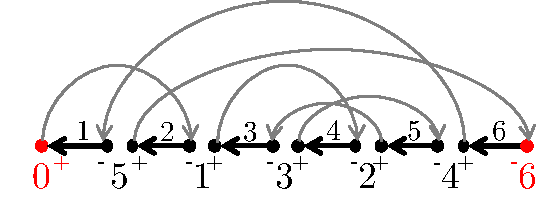
\includegraphics[width=\linewidth]{imagem-ciclo.pdf}
		\caption{Arestas pretas e cinzas}
	\end{subfigure}
	\begin{subfigure}[b]{.4\linewidth}
		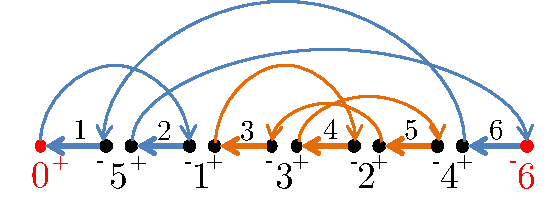
\includegraphics[width=\linewidth]{imagem-ciclo-destacado.pdf}
		\caption{Ciclos destacados}
	\end{subfigure}
	\caption{Grafo de ciclos alternados para a permutação $\pi=(5 \ 1 \ 3 \ 2 \ 4)$.}
	\label{fig:ciclos}
\end{figure}


\subsection{Algoritmos de Ordenação por Reversão}
\label{sec:algoritmos}

Utiliza-se uma variação do algoritmo \textit{Selection Sort} para atacar o problema de ordenação por reversão. O Algoritmo~\ref{alg:selectionSortUsingReversal}, chamado de \textit{Selection Sort Using Reversals} (SSUR), possui um caráter ingênuo, uma vez que realiza sempre o mesmo passo sem se preocupar com outras características da permutação. Além disso, o SSUR não garante a ordenação com o número mínimo de reversões possíveis. Ele inicia pelo elemento 1, verifica a posição atual dele na permutação e faz uma reversão da respectiva posição correta até a posição atual para que o elemento chegue à sua posição correta e, a seguir, repete esses passos para todos os outros elementos até que a permutação esteja ordenada~\cite{Jones}.

Por não garantir o menor número de reversões, o SSUR é um algoritmo de aproximação que não garante uma aproximação melhor do que $(n-1)/2$ vezes a solução ótima. Por exemplo, para a permutação $\pi=(5 \ 1 \ 2 \ 3 \ 4)$ de tamanho $n=5$, o algoritmo SSUR realiza 4 reversões para ordenar $\pi$, porém são necessárias apenas 2 reversões~\cite{Jones}.

\begin{algorithm}[ht]
\Entrada{permutação $\pi$, tamanho da permutação $n$}
\Saida{número de reversões $num\_rev$}
\Inicio{
$num\_rev \ \leftarrow\ 0$; \\
$i \ \leftarrow 1$; \\
\Repita{$\pi =$ identidade ou $i=n-1$}{
    $pos \leftarrow$ posição atual do elemento $i$ na permutação $\pi$ (\textit{e.g.} $\pi_{pos} = i$); \\
    \uSe{$pos \neq i$}{
        $\pi \leftarrow \pi \cdot \rho(i, pos)$; \\
        $num\_rev \leftarrow num\_rev+1$; \\
    }
    $i = i+1$
    }
}
\caption{\textit{Selection Sort Using Reversals}}
\label{alg:selectionSortUsingReversal}
\end{algorithm}

Outro algoritmo utilizado, um pouco mais inteligente que o descrito anteriormente, é conhecido por \textit{Greedy Reversal Sort} (GRS), e está detalhado em Algoritmo~\ref{alg:greedyReversalSort}. O GRS considera os conceitos de \textit{breakpoints} e \textit{strips} crescentes e decrescentes descritos nas Seções~\ref{sec:breakpoints} e~\ref{sec:strips}, respectivamente.

Este algoritmo, por sua vez, possui caráter guloso, pois sempre tenta remover o máximo possível de \textit{breakpoints} a cada passo. Entretanto, também não garante o número mínimo de reversões. O GRS possui garantias matemáticas de que ele remove, em média, um \textit{breakpoint} a cada reversão, ou seja, é capaz de ordenar qualquer permutação $\pi$ em, no máximo, $b(\pi)$ reversões. Porém, como o limite inferior de \textit{breakpoints} que podem ser removidos é dois a cada reversão, temos que o algoritmo exato não conseguiria ordenar $\pi$ em menos do que $b(\pi)/2$ reversões~\cite{Kececioglu}. Portanto, o fator de aproximação do GRS é dado por $\frac{b(\pi)}{b(\pi)/2}=2$.

\begin{algorithm}[ht]
\Entrada{permutação $\pi$, tamanho da permutação $n$}
\Saida{número de reversões $num\_rev$}
\Inicio{
$num\_rev \ \leftarrow\ 0$; \\
\Repita{$\pi =$ identidade}{
    \uSe{$\pi$ tem uma \textit{strip} decrescente}{
    $k \leftarrow$ menor elemento dentre todas as \textit{strips} decrescentes; \\
    $\rho \leftarrow$ reversão que corta na posição depois de $k$ e depois de $k-1$; \\
        \uSe{$\pi \cdot \rho$ não possui \textit{strips} decrescentes}{
        $l \leftarrow$ maior elemento dentre todas as strips decrescentes em $\pi$; \\
        $\rho \leftarrow$ reversão que corta na posição antes de $l$ e antes de $l+1$;
        }
    }
    \uSenao{
    $\rho \leftarrow$ reversão que corta os dois primeiros \textit{breakpoints};
    }
    $\pi \leftarrow \pi \cdot \rho$; \\
    $num\_rev \leftarrow num\_rev+1$
}
}
\caption{\textit{Greedy Reversal Sort}}
\label{alg:greedyReversalSort}
\end{algorithm}

\subsection{Técnicas de Aprendizado de Máquina}

\subsubsection{Regressão Linear}

Regressão Linear (RL) é uma das técnicas mais básicas de regressão que visa quantificar os impactos de variáveis explicativas (ou \textit{features}) em uma variável resposta. O termo \textit{linear} indica a suposição do modelo em que a relação entre a variável resposta e as \textit{features} se dá através de uma combinação linear. Portanto, RL trata-se de um método de aprendizado supervisionado para realizar predições quantitativas.

O modelo de RL múltiplo~\cite{Neter,Bishop} pode ser definido como
\begin{equation}
\label{eq:1}
Y=\beta_0 + \beta_1 x_1 + \beta_2 x_2 + \cdots + \beta_n x_n + \epsilon,
\end{equation}
em que $Y$ representa a variável resposta, $x=\{x_1,x_2,\cdots,x_n\}$ representam as $n$ \textit{features}, $\epsilon$ representa o erro (estocástico) e $\beta=\{\beta_0,\beta_1,\cdots,\beta_n\}$ são os $n+1$ coeficientes de regressão. A estimação desses coeficientes pode ser feita através do método de Mínimos Quadrados, Máxima Verossimilhança, Decomposição QR, Descida do Gradiente e outros métodos~\cite{Neter,Bishop}.

\subsubsection{\textit{Redes Neurais}}

Em busca de obtermos ainda melhores resultados em termos de predição, é possível utilizar abordagens mais complexas, como é o caso das \textit{Redes Neurais} (RN)~\cite{Neter,Bishop}. Na Figura~\ref{fig:arquitetura-nn} apresentamos uma arquitetura de uma RN com uma camada de \textit{input}, uma camada escondida (\textit{hidden}) e uma de \textit{output}. Mais precisamente, os círculos destacados em amarelo representam o \textit{bias} (ou intercepto), e $x=\{x_1,\dots,x_n\}$ (em vermelho) são as $n$ \textit{features} consideradas na análise. Já na camada \textit{hidden} (azul), temos que
\begin{equation}
\label{eq:3}
a^{(2)}=g(X_{m\times (n+1)}W^1_{(n+1)\times h}),
\end{equation}
em que $g(.)$ é uma função de ativação, $X$ é a matriz com o intercepto e todas as $n$ \textit{features} para os $m$ exemplos, e $W^1$ é a matriz com os pesos associados a cada aresta que vai dos $n+1$ neurônios da camada \textit{input} para os $h$ neurônios na camada \textit{hidden}. Por fim, na camada \textit{output} (verde) temos que
\begin{equation}
\label{eq:4}
o=g(u_{m\times (h+1)}W^2_{(h+1)\times c})
\end{equation}
em que $u = (a^{(2)}, I_{m\times1})$, ou seja, adicionamos a coluna do \textit{bias} na matriz $a^{(2)}$ e $W^2$ é a matriz com os pesos associados aos $h+1$ neurônios (já com o intercepto) da camada escondida com os $c$ \textit{outputs}. Note que o número de neurônios na camada \textit{output} está diretamente relacionado com o objetivo da análise que, no caso, seria realizar uma predição e, portanto, teríamos $c=1$.

Arquiteturas mais complexas (isto é, com um maior número de camadas \textit{hidden}) podem ser facilmente estendíveis a partir do exemplo acima. O processo de aprendizado e estimação dos pesos se dá através da etapa de \textit{forward} e de \textit{backpropagation}~\cite{Bishop}. Além disso, técnicas de regularização como o \textit{drop-out}~\cite{Bishop} podem ser utilizadas. No \textit{drop-out}, a cada inserção de um novo vetor de dados na rede, ocorre a eliminação temporária de neurônios e respectivas ligações, com uma determinada probabilidade~\cite{Neter}.

\begin{figure}[ht]
	\centering
	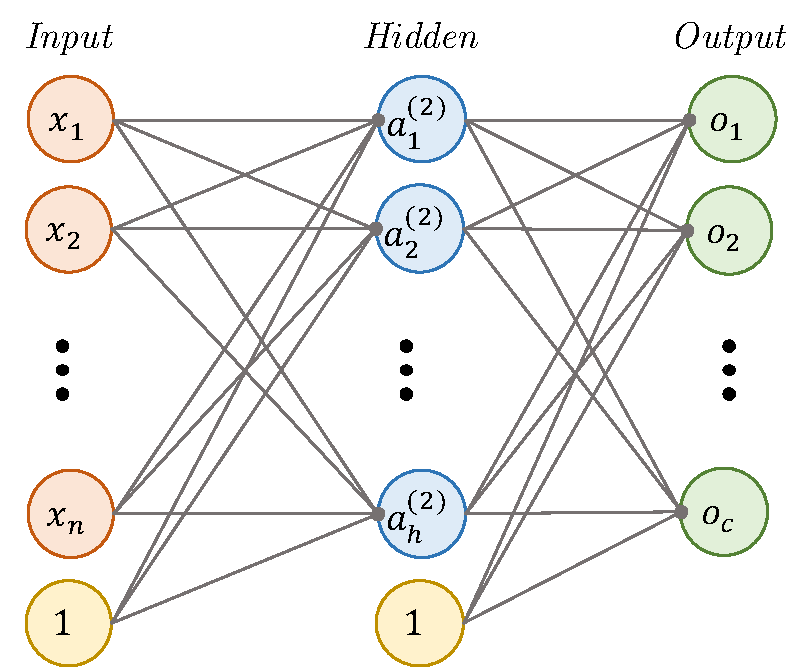
\includegraphics[scale=0.3]{arquitetura-nn.pdf}
	\caption{Arquitetura da Rede Neural com uma camada escondida.}
	\label{fig:arquitetura-nn}
\end{figure}

\section{Metodologia}

Dadas todas as definições e nomenclaturas necessárias, a base desse projeto é construir um modelo baseado em técnica de AM que seja capaz de estimar a distância de reversão, baseando-se em algumas \textit{features} extraídas das permutações. O treinamento dos algoritmos será feito considerando permutações de tamanhos reduzidos e, então, avaliaremos a sua qualidade em permutações grandes.

\subsection{Conjunto de dados}

O conjunto de dados utilizado neste projeto considera todas as permutações de tamanho $n = \{5,6,\cdots,10\}$, totalizando $4.037.880$ permutações. Para cada permutação, foi calculado um vetor de 13 \textit{features}, bem como a distância exata de reversão\footnote{A distância exata de reversão foi, parte extraída do site \url{http://mirza.ic.unicamp.br/} e, também, parte fornecida pelo prof. Dr. Zanoni Dias do IC-UNICAMP.}. A Tabela~\ref{tab:1} mostra todas as \textit{features} calculadas e a distância exata de reversão, exemplificadas com a permutação $\pi = (5\ 4\ 3\ 1\ 2)$.

\begin{table*}[ht]
	\centering
	\caption{Exemplo das \textit{features} que foram utilizadas para o treinamento dos algoritmos de AM para a permutação $\pi = (5\ 4\ 3\ 1\ 2)$}
	\label{tab:1}
	\begin{tabular}{lc}
		\toprule
		\textit{Feature} & Valor observado para $\pi$\\ 
		\midrule
		Quantidade de \textit{breakpoints} & 3 \\
    	Quantidade de \textit{strips} unitárias & 2 \\ 
    	Tamanho da menor \textit{strip} & 2 \\
    	Tamanho da maior \textit{strip} & 3 \\
    	Quantidade de \textit{strips} crescentes & 3 \\
    	Quantidade de \textit{strips} decrescentes & 1 \\
    	Total de ciclos & 2 \\
    	Quantidade de ciclos impares & 2 \\
    	Quantidade de ciclos unitários & 1 \\
    	Tamanho do maior ciclo & 5 \\
    	Tamanho do menor ciclo & 5 \\
    	Quantidade de ciclos orientados & 1 \\
    	Tamanho da permutação & 5 \\
    	\midrule
    	Distância exata & 2\\
		\bottomrule
	\end{tabular}
\end{table*}

Sabe-se que, em técnicas que envolvem AM, problemas a se evitar são o de \textit{underfitting} e \textit{overfitting}. Como uma tentativa de evitar e avaliar tais problemas, podemos dividir o nosso conjunto de dados em: treino, validação e teste~\cite{Neter,Bishop}. Inicialmente, o \textit{dataset} foi dividido em dois, uma parcela de 80\% e outra de 20\%. A parcela de 20\% é reservada para o conjunto de teste, enquanto que os outros 80\% são dividimos novamente em 80\% para treinamento e 20\% para validação.

\subsection{\textit{Workflow} da Metodologia}

A Figura~\ref{fig:workflow} ilustra o fluxograma deste trabalho. Inicialmente, para todas as permutações de tamanho $n=\{5,6,\cdots,10\}$, foram  extraídas as \textit{features} apresentadas na Tabela~\ref{tab:1}, bem como a distância exata de reversão. Em seguida, esse conjunto de dados foi dividido em treino, validação e teste, de modo que os conjuntos de treino e validação foram utilizados para o treinamento e análise de \textit{overfitting} dos modelos. Posteriormente, após os melhores modelos serem escolhidos, em termos de algumas medidas estatísticas como, por exemplo, o \textit{Root Mean Squared Error} (RMSE), aplicamos o conjunto de testes e também um conjunto de permutações de tamanho $n=\{11,20,30,\cdots,100\}$ sendo que, para cada $n$, consideramos uma amostra de 5000 permutações. Por fim, comparamos os modelos com os Algoritmos~\ref{alg:selectionSortUsingReversal} e~\ref{alg:greedyReversalSort} descritos na Seção~\ref{sec:algoritmos}.

\begin{figure}[H]
	\centering
	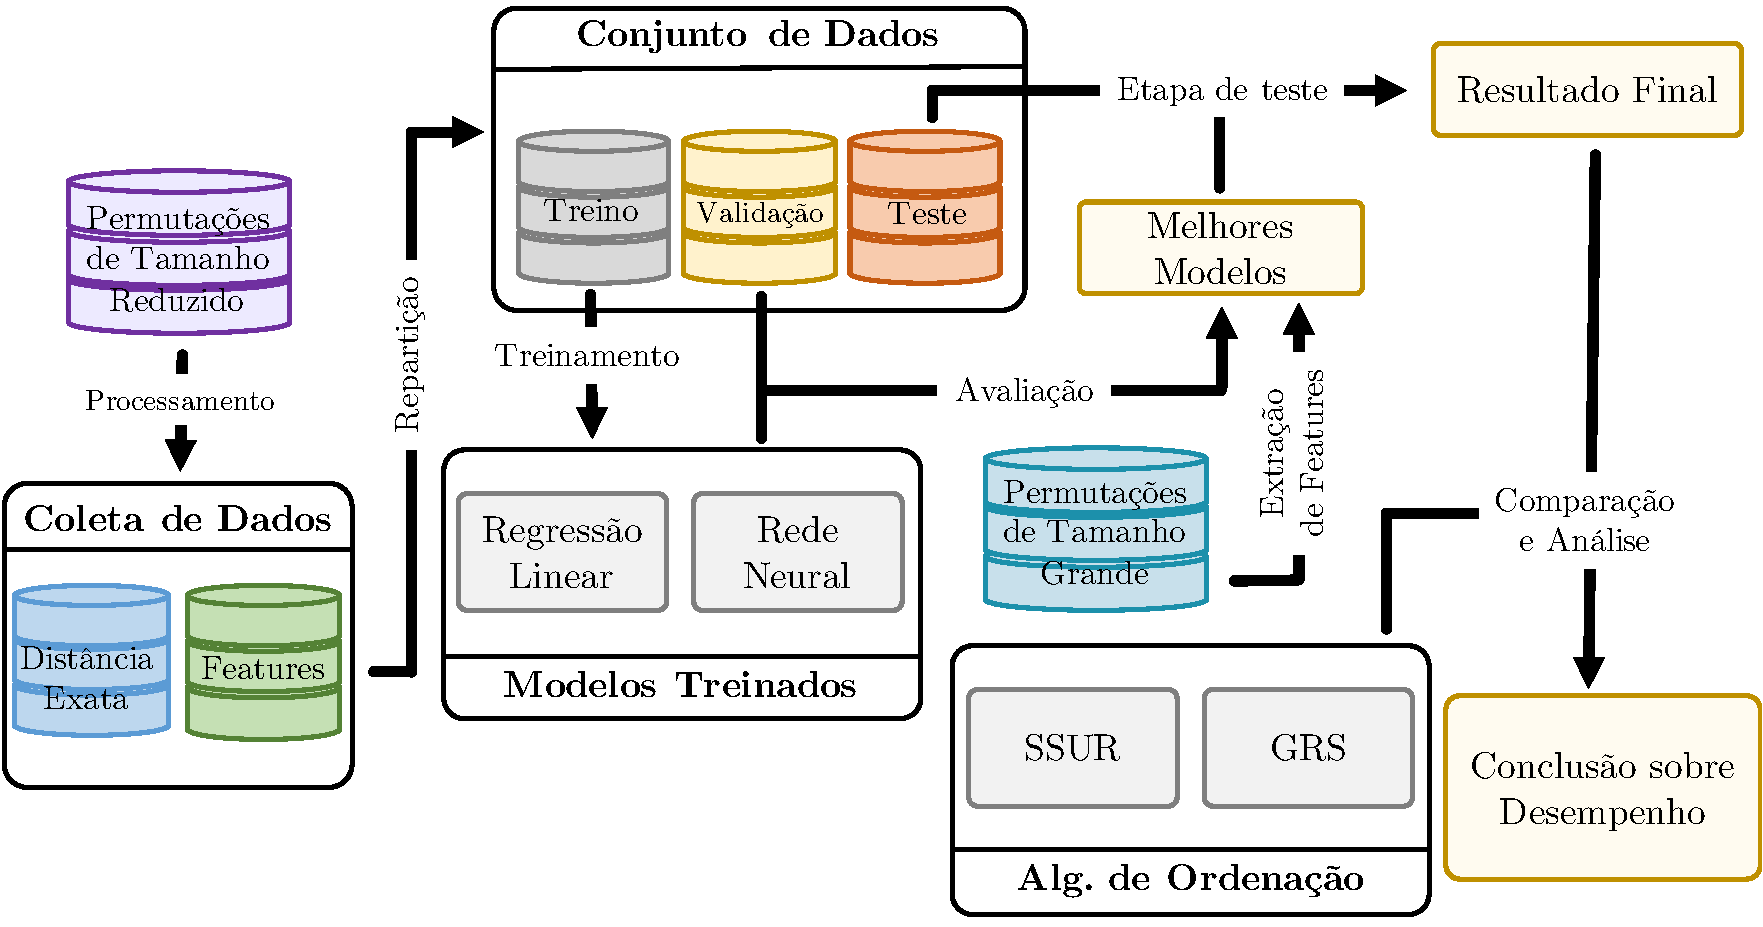
\includegraphics[width=1\textwidth]{workflow.pdf}
	\caption{Fluxograma da metodologia do projeto.}
	\label{fig:workflow}
\end{figure}

\section{Resultados e Avaliação}
\label{sec:resultados}

Para a estimação dos parâmetros da RL, foi considerado a decomposição QR. Já na RN, foram consideradas as arquiteturas descritas na Tabela~\ref{tab:2}, como função de ativação foi utilizada a ReLU~\cite{Bishop} e como função de custo o \textit{Mean Squared Error}~\cite{Neter}.  

A Tabela~\ref{tab:2} também mostra o RMSE dos conjuntos de validação (RMSE$_{val}$) para cada modelo considerado. Pode-se observar que, dentre todos os modelos, o que obteve menor RMSE$_{val}$ foi a RL e, com relação aos modelos de RN, a rede I-RN B foi a que apresentou melhores resultados. Desse modo, por parcimônia, a análise seguirá com os modelos RL e I-RN B.

\begin{table}[ht]
	\centering
	\caption{Modelos utilizados na etapa de treinamento, bem como o valor do RMSE$_{val}$ para cada um dos modelos}
	\label{tab:2}
	\begin{tabular}{cccccc}
		\toprule
		& \multicolumn{2}{c}{1a \textit{Hidden}} & \multicolumn{2}{c}{2a \textit{Hidden}} & \\
		\cmidrule(lr){2-3} \cmidrule(lr){4-5}
		Modelo & $\eta^1$ & $\delta^1$ & $\eta^2$ & $\delta^2$ & RMSE$_{val}$\\ 
		\midrule
		I-RN A & 15 & 0.2 & -- & -- & 0.5055\\ 
		I-RN  B & 30 & 0.2 & -- & -- & \textbf{0.4866}\\ 
		II-RN A & 30 & 0.3 & 15 & 0.2 & 0.5184\\
		II-RN B & 64 & 0.3 & 32 & 0.2 & 0.4973\\
		II-RN C & 256 & 0.3 & 128 & 0.2 & 0.4899\\
		\midrule
		RL & -- & -- & -- & -- & \textbf{0.4814}\\
		\bottomrule
	\end{tabular}
	\begin{tablenotes}\footnotesize
			\item{Características que não se aplicam estão indicadas com --. Além disso, $\eta^i$ e $\delta^i$ fazem referencia ao número de neurônios e ao valor do \textit{drop-out} na camada escondida $i$, respectivamente.}
	\end{tablenotes}
\end{table}

A Tabela~\ref{tab:3}, por sua vez, apresenta os valores de RMSE dos conjuntos de teste (RMSE$_{teste}$) e novamente o RMSE$_{val}$ para os modelos RL e I-RN B. Como o valor de RMSE$_{val}$ é muito próximo ao valor de RMSE$_{teste}$, pode-se conjecturar que não houve \textit{overfitting} em nenhum dos modelos.

\begin{table}[ht]
	\centering
	\caption{RMSE para o modelo de RL e RN, considerando o conjunto de validação e teste}
	\label{tab:3}
	\begin{tabular}{ccc}
		\toprule
		Modelo & RMSE$_{val}$ & RMSE$_{teste}$ \\ 
		\midrule
		RL & 0.4814 & 0.4813 \\ 
		I-RN B & 0.4866 & 0.4867 \\ 
		\bottomrule
	\end{tabular}
\end{table}

Na Figura~\ref{fig:bp} é possível observar o gráfico da distância média \textit{vs} o número de \textit{breakpoints} e também o gráfico da distância média \textit{vs} o tamanho da permutação para os modelos RL, I-RN B e para os algoritmos SSUR (Alg.~\ref{alg:selectionSortUsingReversal}) e GRS (Alg.~\ref{alg:greedyReversalSort}), considerando permutações de tamanho reduzido, ou seja, $n \in \{5, \ 6, \ 7, \ 8, \ 9, \ 10\}$ para o conjunto de teste. 

\begin{figure}[H]
	\centering
	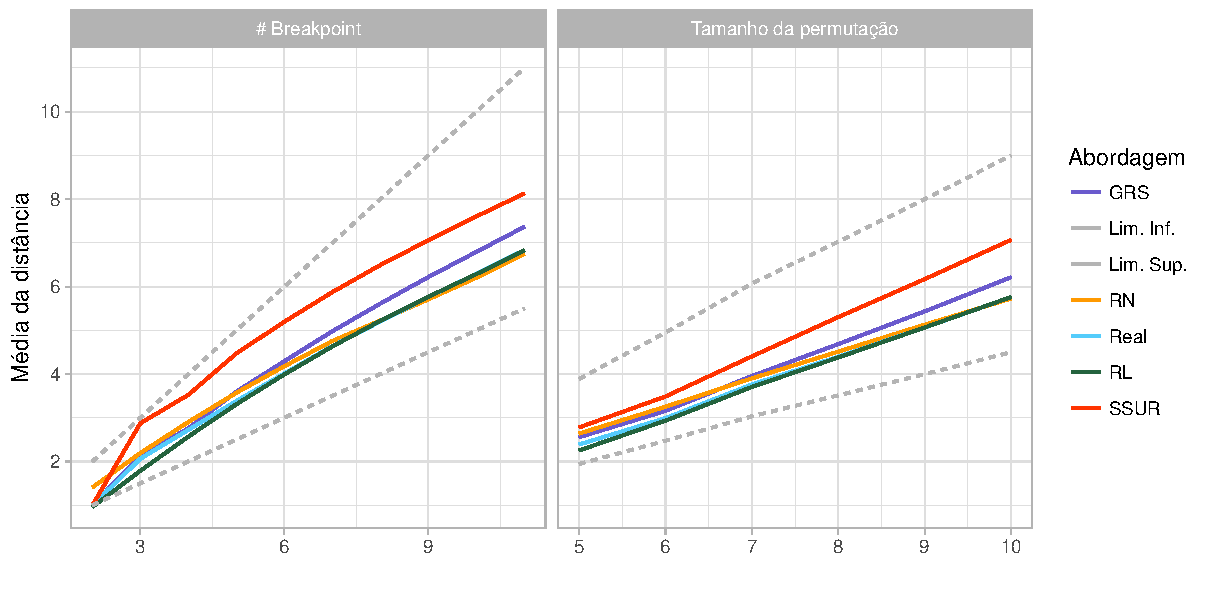
\includegraphics[scale=0.5]{bp.pdf}
	\caption{Distância média \textit{vs} o número de \textit{breakpoints}, bem como a distância média \textit{vs} o tamanho da permutação.}
	\label{fig:bp}
\end{figure}

Observa-se nos dois gráficos que, para todas as abordagens, a média ficou dentro dos limites inferior e superior. Mais precisamente, nota-se que o algoritmo SSUR foi o que se distanciou mais dos valores exatos de distância de reversão, representados pela reta Real (cor azul) e que o algoritmo de 2-aproximação (GRS) manteve-se sempre próximo do valor exato. Por outro lado, percebe-se que os melhores resultados estão nas abordagens propostas de AM, sendo que a RL foi a que se manteve mais próxima da reta dos valores exatos, embora a RN também tenha apresentado resultados satisfatórios. Por fim, é possível observar que, à medida em que o número de \textit{breakpoints} e o tamanho da permutação cresce, maior é a distância média e, mais próximo do valor exato as abordagens de AM ficam.

A Figura~\ref{fig:dist} apresenta a diferença, em módulo, das curvas da Figura~\ref{fig:bp} em relação a curva Real. Os resultados corroboram com o que foi discutido anteriormente, ou seja, o algoritmo GRS, a RL e a RN foram as abordagens que apresentaram resultados mais próximos do valor exato de distância de reversão, fato observado pelos menores valores de diferença entre as retas. Percebe-se, também, que a RL e a RN foram as que obtiveram a menor distância e que, conforme o número de \textit{breakpoints} e o tamanho da permutação aumenta, menor é a diferença para esses dois modelos.

\begin{figure}[H]
	\centering
	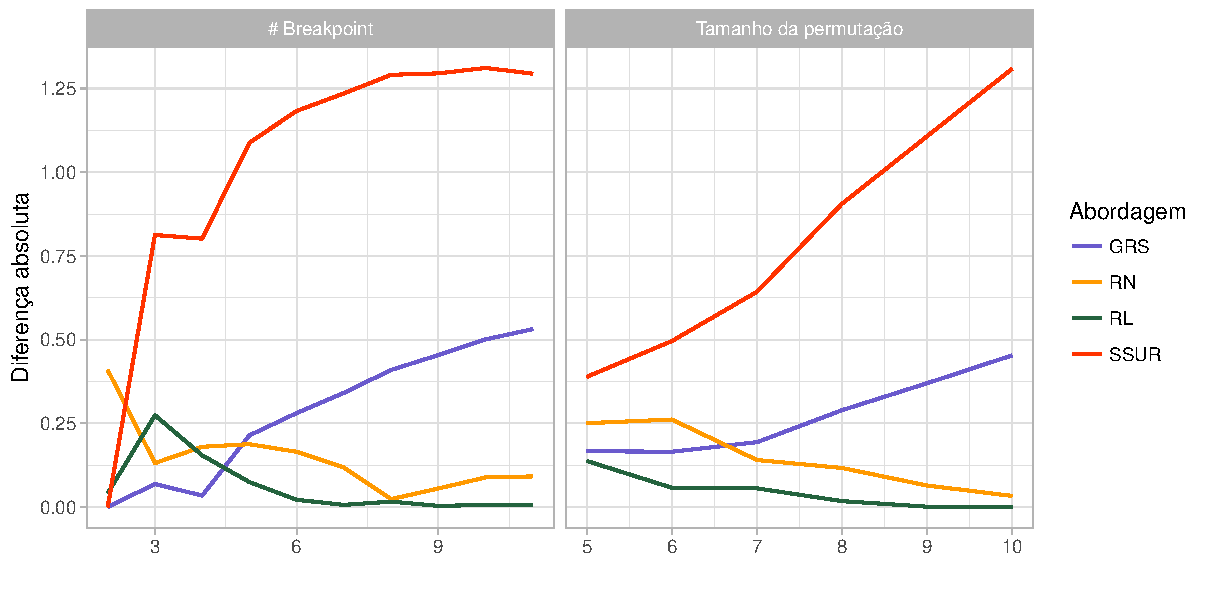
\includegraphics[scale=0.5]{dist.pdf}
	\caption{Diferença, em módulo, das curvas da Figura~\ref{fig:bp} com a curva real.}
	\label{fig:dist}
\end{figure}

Visto que os resultados das abordagens de AM foram satisfatórios, torna-se interessante verificar a proporção de distâncias que possam ter sido superestimadas ou subestimadas. A Tabela~\ref{tab:4} mostra a proporção da distância de reversão que foi calculada fora dos limites inferior ($\frac{b(\pi)}{2}$) e superior ($b(\pi)$) para todas as abordagens considerando apenas as permutações de tamanho reduzido. Como era esperado, o GRS foi o único que não apresentou resultados fora dos limites. Já o SSUR, apresentou uma quantidade significativa de estimações fora do limite superior, evidenciando que esse algoritmo superestima a distância de reversão, ou seja, realiza muito mais operações do que a quantidade necessária. Nas abordagens de AM, embora não houvesse garantia nenhuma de obter estimações dentro dos limites, nota-se que, apesar de existirem casos fora dos limites, a proporção observada de ocorrência desses é de fato muito baixa, indicando novamente uma boa qualidade na estimação de permutações com tamanho reduzido.

\begin{table}[H]
	\centering
	\caption{Proporção da distância de reversão que foi calculada fora dos limites inferior ($\frac{b(\pi}{2}$) e superior ($b(\pi)$) para as permutações de tamanho reduzido}
	\label{tab:4}
	\begin{tabular}{ccccc}
		\toprule
		&  \multicolumn{4}{c}{Abordagem}\\
		\cmidrule(lr){2-5}
		Limite & GRS & SSUR & RL & RN \\ 
		\midrule
		Inferior & 0 & 0 & $2\times10^{-5}$ & $1\times10^{-6}$\\ 
		Superior & 0 & 0.0208 & 0 & 0 \\ 
		\bottomrule
	\end{tabular}
\end{table}

Considerando os resultados interessantes obtidos para as permutações de tamanho reduzido, decidiu-se por analisar o comportamento das abordagens para permutações de tamanhos maiores, considerando $n\in\{11,20,30,\cdots,100\}$.
A Figura~\ref{fig:big} apresenta a distância média \textit{vs} o número de \textit{breakpoints}, bem como a distância média \textit{vs} o tamanho da permutação para as permutações maiores. De modo geral, nota-se que todas as abordagens permaneceram dentro ou próximo dos limites superior e inferior. Novamente, observa-se que o SSUR apresentou o maior valor para a distância média, seguido do GRS. A RN apresentou valores bem menores do que os outros métodos, sinalizando uma possível subestimação, ou seja, estimando valores menores do que eles deveriam ser. Em relação a RL, observou-se que as estimações ficam próximas da média entre os limites superior e inferior. É importante ressaltar que, para uma melhor análise, seria necessário comparar os resultados obtidos com os valores exatos da distancia de reversão, uma tarefa que, computacionalmente, se torna inviável.

\begin{figure}[H]
	\centering
	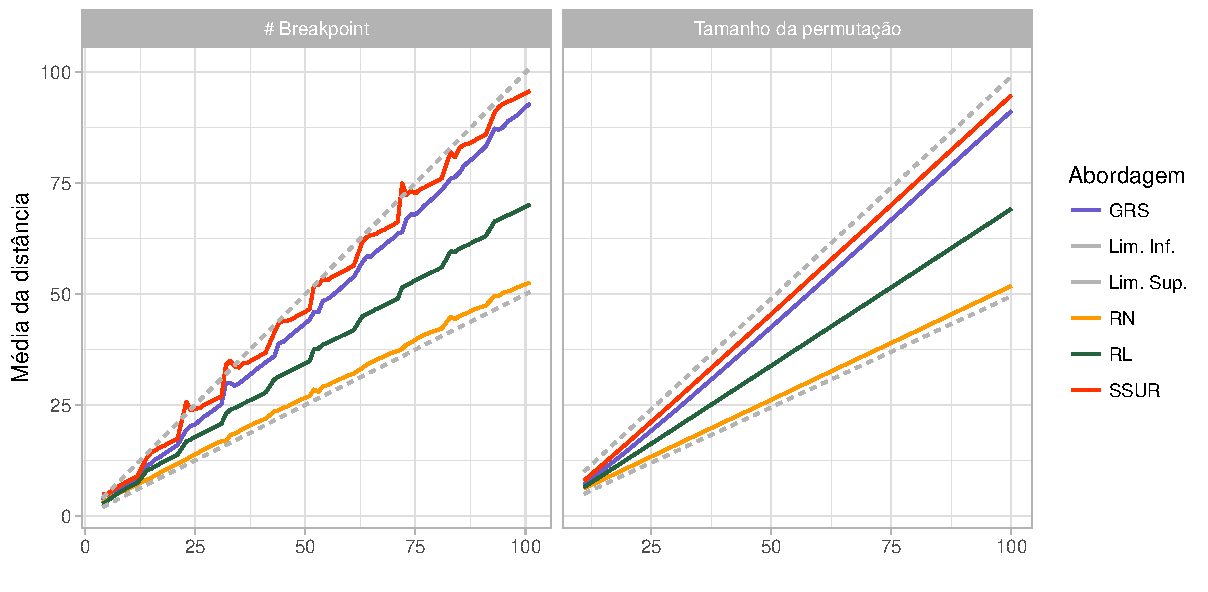
\includegraphics[scale=0.5]{big.pdf}
	\caption{Distância média \textit{vs} o número de \textit{breakpoints}, bem como a distância média \textit{vs} o tamanho da permutação, para permutações maiores.}
	\label{fig:big}
\end{figure}

 Por fim, a Tabela~\ref{tab:5} apresenta a proporção da distância de reversão que foi calculada fora dos limites inferior ($\frac{b(\pi)}{2}$) e superior ($b(\pi)$) para todas as abordagens considerando as permutações de tamanho maior. Novamente, como era esperado, o GRS não apresentou resultados fora dos limites. Já o SSUR, apresentou estimações fora do limite superior, evidenciando que esse algoritmo superestima a distância de reversão, ratificando o que foi discutido anteriormente. Nas abordagens de AM, a RL apresentou todos os resultados dentro dos limites. Já na RN, vemos uma quantidade não desprezível de estimações fora do limite inferior, comprovando uma possível subestimação.

\begin{table}[H]
	\centering
	\caption{Proporção da distância de reversão que foi calculada fora dos limites inferior ($\frac{b(\pi}{2}$) e superior ($b(\pi)$) para as permutações com tamanho maior}
	\label{tab:5}
	\begin{tabular}{ccccc}
		\toprule
		&  \multicolumn{4}{c}{Abordagem}\\
		\cmidrule(lr){2-5}
		Limite & GRS & SSUR & RL & RN \\ 
		\midrule
		Inferior & 0 & 0 & 0 & $0.0333$\\ 
		Superior & 0 & $0.0096$ & 0 & 0 \\ 
		\bottomrule
	\end{tabular}
\end{table}

\section{Problemas encontrados}
\label{sec:problemas}
Neste trabalho, tentou-se implementar o algoritmo de Christie~\cite{Christie} com o objetivo de utilizá-lo na comparação e até mesmo extrair das permutações outras \textit{features} para os modelos de AM. 

Apesar do algoritmo de 1,5-aproximação apresentar menor complexidade de entendimento se comparado ao de 1,375, enfrentou-se grande dificuldade em implementar algumas partes do algoritmo, porque alguns passos são omitidos, por exemplo, o passo que determina como é realizada a conexão de arestas pretas e cinzas no grafo de ciclos; outros passos não estão explicados de forma clara, como o que define as reversões que os vértices no grafo de reversões representam. 

Apesar de Christie ter publicado uma \textit{errata}~\cite{ChristieERR} para o seu artigo original~\cite{Christie} melhorando a explicação de alguns detalhes, os passos citados anteriormente continuaram sem uma definição clara. Além disso, Soncco-Álvarez e Ayala-Rincón~\cite{Soncco}, em 2012, identificaram e corrigiram um problema no principal lema que define a transformação do grafo de reversões.

Considerando os empecilhos encontrados e o vasto tempo despendido tentando implementar tal algoritmo, seria relevante aprofundar os conhecimentos na área a fim de conseguir solucionar completamente as imprecisões do algoritmo em questão e assim implementá-lo de forma correta.


\section{Conclusões}
\label{sec:conclusoes}
    
Este trabalho analisou a aplicação de métodos de Aprendizado de Máquina, mais especificamente Regressão Linear (RL) e Redes Neurais (RN), na estimação da distância de reversão para permutações sem orientação de genes, problema que foi comprovado pertencer a classe NP-Difícil. Esses métodos foram comparados com algoritmos já estabelecidos na literatura (SSUR e GRS) e também com a distância exata de reversão.

Os resultados descritos na seção anterior mostraram que a utilização de RL apresenta resultados melhores ou tão bons quanto o algoritmo de 2-aproximação (GRS). Para as permutações de tamanhos 8, 9 e 10, a RL praticamente se equiparou a curva de distância exata a menos de uma diferença ínfima observada nos gráficos da Figura~\ref{fig:dist}. Já a abordagem de RN superestimou a distância de reversão para permutações de tamanho 5 e 6 se comparado ao algoritmo GRS, mas para os outros tamanhos de permutação, ou seja, 7, 8, 9 e 10, esta abordagem mostrou uma melhor estimação que o GRS e pior ou no máximo semelhante à abordagem de RL.

Para as permutações de tamanho maior que 10, a RL e RN se mostraram promissoras, porém acredita-se que os modelos necessitam de mais \textit{features} para a etapa de treinamento, bem como maior potencial computacional para arquiteturas de RN mais complexas. Em RN, uma quantidade significativa de estimações ficou fora do limite inferior, o que confirma a afirmação anterior. Além disso, uma comparação com os valores exatos das permutações grandes poderia permitir uma análise mais precisa.

A utilização de modelos de AM, se mostrou uma interessante ferramenta para se estimar a distância de reversão entre permutações. Para melhorar a análise, como trabalho futuro seria interessante testar outros modelos de AM e também adicionar à comparação um algoritmo melhor que o SSUR e GRS, como o de 1,5-aproximação proposto por Christie~\cite{Christie} ou até mesmo o de 1,375-aproximação proposto por Berman \textit{et al.}~\cite{Berman}.

\bibliographystyle{splncs}
\bibliography{library}

\end{document}